\setcounter{pageFix}{\value{page}}
\begin{abstract}
\thispagestyle{fancy}
    \setcounter{page}{\value{pageFix}}
        \addcontentsline{toc}{section}{Abstract}
    Recent analysis \citep{McGaugh2016} of the SPARC galaxy sample found a
    surprisingly tight relation between the radial acceleration inferred from
    the rotation curves, and the acceleration due to the baryonic components of
    the disc.  It has been suggested that this relation may be evidence for new
    physics, beyond $\Lambda CDM$.  In this letter we show that the 18
    galaxies from the MUGS2 match the SPARC acceleration relation. These
    cosmological simulations of star forming, rotationally supported discs were
    simulated with a {\sc WMAP3} $\Lambda CDM$ cosmology, and match the SPARC
    acceleration relation with less scatter than the observational data.  These
    results show that this acceleration law is a consequence of
    dissipative collapse of baryons, rather than being evidence for exotic
    dark-sector physics or new dynamical laws.
\end{abstract}

\section{Introduction}
For nearly a century, observations of kinematics in galaxies and clusters of
galaxies have found large velocities inconsistent with the luminous matter
within them.  Even when thorough, comprehensive surveys of the baryonic mass
within galaxies and clusters have been performed, most of the matter has been
found to be missing.  \citet{Zwicky1937} presented observations of galaxy
velocity dispersions in the Coma cluster, and proposed that the bulk of that
cluster's mass was some sort of dark matter (DM).  Later, the groundbreaking
observations of \citet{Rubin1970} showed that this dark matter was also
ubiquitous within disc galaxies like our own.  Today, there is a wealth of
evidence for cold dark matter, not just from galaxy kinematics, but from the
formation of large-scale structure \citep{Blumenthal1984}, the cosmic microwave
background power spectrum \citep{Planck2014},  and the primordial abundances of
elements after Big Bang Nucleosynthesis \citep{Walker1991}.  Dark matter is now
part of the standard cosmology, $\Lambda CDM$, in which most of the
matter in our universe is in fact dark.  Despite this, we still do not know the
actual form that dark matter particles take.  Both direct detection experiments
and searches for dark matter annihilation have failed to conclusively observe
these particles \citep{Aprile2012}, and as such, alternative explanations for
the kinematics of galaxies have been proposed.

The Spitzer Photometry \& Accurate Rotation Curves (SPARC) sample, presented in
\citet{Lelli2016} is a new set of observations and derived mass models for a large
number of rotation-dominated galaxies.  By using $3.6\mu m$ observations, the
stellar mass can be estimated with great accuracy.  The stellar mass is
complemented with $21 cm$ observations of {\sc HI} to get a measure of the gas
mass within the disc. The recent paper by \citet{McGaugh2016}
analyzed this sample, and determined a relation between the observed radial
acceleration determined from the rotation curve ($g_{obs}$), and the
acceleration induced by the baryons observed in the disc ($g_{bar}$).
\citet{McGaugh2016} found that for large values of $g_{bar}$, $g_{obs}\sim
g_{bar}$, while for values of $g_{bar} \lesssim 10^{-10} m\;s^{-2}$, the observed
acceleration begins to rapidly outstrip the acceleration one would expect from
the observed baryons.  They find that the relation between $g_{bar}$ and
$g_{obs}$ is well fit by:
\begin{equation} \label{g_fit}
    g_{obs} = \frac{g_{bar}}{1-\exp{(-\sqrt{g_{bar}/g_\dagger})}},
\end{equation}
where $g_\dagger=1.20\pm 0.26\times10^{-10}\;ms^{-2}$.  In addition to the
simple functional form, \citet{McGaugh2016} find a surprisingly low scatter in
this relation, with residuals normally distributed with $\sigma =
0.11\;\mathrm{dex}$.  The authors noted that this is the same functional form as
the Modified Newtonian Dynamics (MOND) \citep{Milgrom1983} acceleration law,
which attempts to explain galaxy rotation curves without DM.

In discussing these results, \citet{McGaugh2016} offer three possible
explanations for the tight relation. 
\begin{enumerate}
    \item The end point of galaxy formation with conventional (baryonic?)
        physics.
    \item New dark sector physics coupling dark matter and baryons
    \item New dynamical laws (such as MOND
        Tensor-Vector-Scalar Gravity (TeVeS)
        \citep{Bekenstein2004}, etc.)
\end{enumerate}

This is not the first set of observations that appear to be in discordance with
$\Lambda CDM$.  N-body simulations of halo formation have found DM halos follow
a universal, ``cuspy'' density profile \citep{Navarro1996}.  Yet observations of
dwarf galaxies in the local universe find flat, ``cored'' central densities (the
``cusp-core problem'', \citealt{Walker2011}).  Meanwhile, DM-only simulations
were finding that the local group should contain thousands of dwarfs, in
contrast to the dozens actually observed (the ``missing satellites problem''
\citealt{Klypin1999}).  Many of these halos are large enough that suppression of
star formation by reionization could not explain their absence from the
observations (the ``too big to fail'' problem \citealt{Boylan-Kolchin2011}).  

A common feature in each of these conflicts is the comparison of observations to
simulations of galaxy formation that rely purely on N-body, DM-only simulations.
We now know that the impact of baryonic physics, chief among them the feedback
from massive stars and black holes, can have a dramatic effect on the star
formation history (e.g. \citealt{Keller2015}) and density profile of galaxies
\citep{Mashchenko2006}.  Multiple studies \citep[etc]{Pontzen2012,Sawala2016}
have found these problems disappear when galaxies are simulated with gas
dynamics, along with reasonable models for star formation, radiative cooling,
and stellar feedback.  This is what constitutes a modern theory of galaxy
formation, the first of the three options offered to explain the SPARC
acceleration relation.  Galaxies are formed through the gravitational collapse
of collisional particles (gas) into a rotationally supported disc.  Conservation
of angular momentum, combined with star formation and feedback within that disc,
leads to the observed scaling relations and galaxy properties we see today.
Whether this can also reproduce the SPARC acceleration relation has been yet to
be demonstrated.

In this letter, we show that the apparent tension between models of galaxy
formation in $\Lambda CDM$ and the SPARC observations also evaporates when the
collisional collapse of baryons is taken into account.  We find that the
$g_{obs}-g_{bar}$ relation for a set of pre-existing cosmological galaxy
simulations, evolved in a conventional $\Lambda CDM$ cosmology, matches the
SPARC acceleration law, with even tighter scatter than the observed sample.

\section{The MUGS2 Sample}
The McMaster Unbiased Galaxy Simulations 2 (MUGS2) sample is an unbiased,
statistically representative set of 18 cosmological zoom-in simulations of $L*$
disc galaxies.  These galaxies were simulated in a {\sc WMAP3} $\Lambda CDM$
cosmology, with parameters $H_0 = 73\kms \Mpc^{-1}$, $\Omega_M=0.24$,
$\Omega_{bar}=0.04$, $\Omega_\Lambda=0.76$, and $\sigma_8=0.76$.  The MUGS2
$z=0$ halo masses range from $3.7\times10^{11}\Msun$ to $2.2\times10^{12}\Msun$,
with disc masses ranging from $1.8\times10^{10}\Msun$ to
$2.7\times10^{11}\Msun$.  For more details on the creation of the MUGS2 initial
conditions, see the original MUGS paper, \citet{Stinson2010}.  For more
information on the simulations themselves, see \citet{Keller2015,Keller2016a}.

MUGS2 was simulated using the modern smoothed particle hydrodynamics code {\sc
Gasoline} \citep{Wadsley2004,Keller2014}.  The simulations used metal line
radiative cooling \citep{Shen2010}, as well as a simple Schmidt law for star
formation.  What sets MUGS2 apart from the original MUGS, aside from improved
hydrodynamics, is the use of a physically motivated, first principles model for
treating feedback from supernovae. (SNe).  Originally presented in
\citet{Keller2014}, the superbubble model captures the effects of thermal
conduction and evaporation between a hot, SNe heated bubble and a surrounding
shell of cold, swept-up interstellar medium (ISM).  This model was derived to allow unresolved
superbubbles to radiatively cool at realistic rates, with no free parameters,
while automatically capturing the effects of clustered SNe.

\subsection{Calculating Accelerations from MUGS2}
In order to compare to the SPARC sample, we located the central halos using the
AMIGA halo finder \citet{Knollmann2009}.  We center the halos using the
shrinking sphere method described in \citet{Power2003}.  Next, in order to
measure rotation curves of the galaxies face-on, we calculate the net angular
momentum vector of all gas within $10\kpc$ of the center of the disk, and rotate
our simulations such that this vector is orthogonal to the x-y plane.
Accelerations were measured in 100 circular annuli $300\pc$ thick.
Accelerations were then calculated using a direct N-body summation on all of the
particles in the halo on those particles within the annulus.  Only the in-plane
component of the acceleration was used, to better follow \citet{McGaugh2016}.
For $g_{obs}$ (the observed acceleration), all particles (gas, stars, and DM)
within the simulation were used.  To calculate $g_{bar}$, we simply calculate
the contributions from stars and gas, $g_*$ and $g_{gas}$, so that
$g_{bar}=g_*+g_{gas}$.  For each of $g_*$ and $g_{gas}$, we use a direct
summation only on those particles (stars and gas respectively).  This process of
direct summation to calculate gravity is equivalent to the numerical solution to
Poisson's equation used in \citep{McGaugh2016}.  The mass model in SPARC
\citep{Lelli2016} included stellar masses estimated from $3.6\;\mu\rm{m}$ near
infrared observations, and gas masses estimated using $21\;\rm{cm}$ observations
of {\sc HI}.  These {\sc HI} masses were converted to total gas masses 
using the simple equation $M_{gas}=1.33M_{HI}$.  Rather than using the total gas
mass from our simulations, we match the {\sc HI}-based estimate from SPARC by
calculating accelerations due to gas using $1.33M_{HI}$, rather than $M_{gas}$.
This is especially important near the outskirts of the galaxy, where the
contribution to the baryonic mass from ionized gas in the ISM and circumgalactic
medium is most significant.  The HI fraction is calculated using the radiative
cooling code within {\sc Gasoline}, which relies on tabulated equilibrium
cooling rates from {\sc CLOUDY} \citep{Ferland2013}.

\begin{figure}
    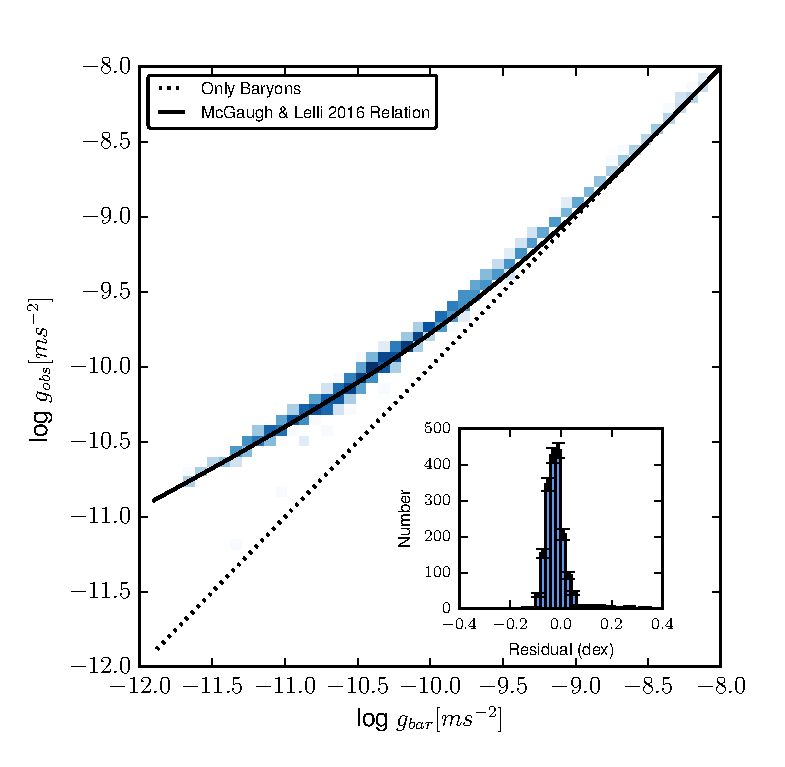
\includegraphics[width=0.9\textwidth]{figures4/SPARC_plot.eps}
    \caption[Total acceleration vs. baryonic acceleration in MUGS2]{Total
    acceleration ($g_{obs}$) vs acceleration due to baryons ($g_{bar}$) from
    1800 data points in the $z=0$ MUGS2 sample, shown in the blue 2-dimensional
    histogram.  The dotted black curve shows the 1:1 relation expected if the
    acceleration was due to baryons alone (without dark matter), while the solid
    line shows the relation presented in \citet{McGaugh2016}.  A Gaussian
    distribution fitted to these residuals finds a variance of $\sigma=0.05$
    dex, significantly lower than the 0.11 dex found by \citet{McGaugh2016}.}
    \label{SPARC_plot}
\end{figure}
\section{Results}
\subsection{z=0 Acceleration Relation}
The MUGS2 sample gives us 1800 acceleration data points, just over 2/3 the
sample size of \citet{McGaugh2016}. We show in figure~\ref{SPARC_plot} the
$g_{obs}-g_{bar}$ relation for the MUGS2 sample, compared both to the pure
baryonic acceleration and the SPARC acceleration relation.  It is clear these
simulated galaxies follow the \citet{McGaugh2016} relation {\it extremely} well.
As can be seen from the inset residual distribution, our simulated galaxies
follow the SPARC relation even more tightly than the actual observational data.
The scatter we do see, with $\sigma=0.05$ dex, is consistent with the
\citet{McGaugh2016} estimates.  They decomposed their scatter of $0.11$
dex into different sources, and when all of the observational uncertainties are
removed, the remaining intrinsic scatter gives a variance of $\sigma=0.06$ dex,
very close to the value we find here.  A reduced $\chi^2$ statistic of the SPARC
relation fit to the $z=0$ MUGS2 data finds a very good fit, with $\chi^2_\nu =
1.25$.  These simulation data are fit by equation~\ref{g_fit} at least as well
as the original SPARC data.

\subsection{Feedback \& the Evolution of the Acceleration Relation}
\begin{figure}
    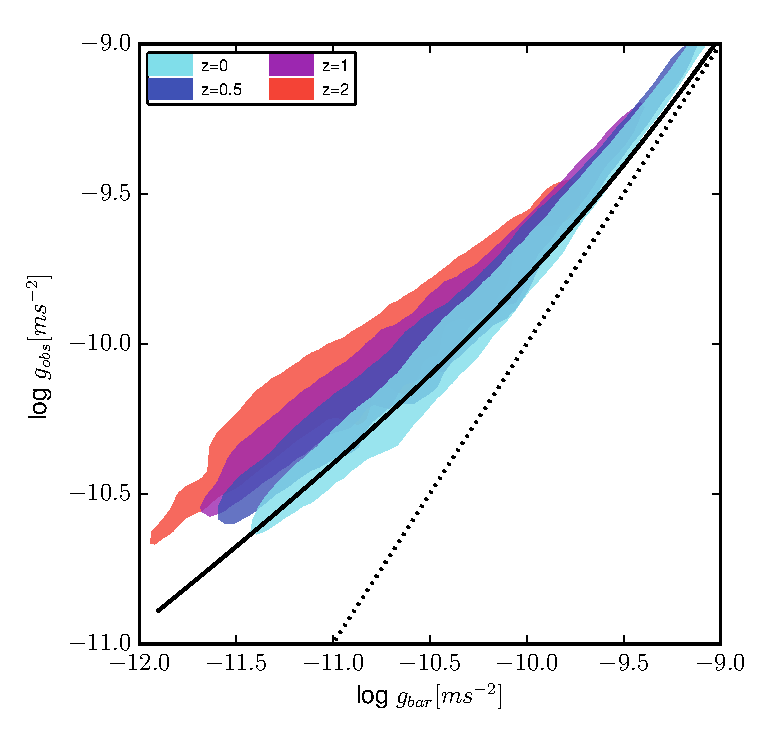
\includegraphics[width=0.6\textwidth]{figures4/redshift_evolution.eps}
    \caption[Redshift evolution of acceleration relation]{The  simulated
    $g_{obs}-g_{bar}$ relation is not constant with redshift.  As this figure
    shows, at higher redshift the low $g_{bar}$ slope is much shallower than at
    $z=0$.  This shows that for high redshift galaxies, their discs can be
    depleted of baryons compared with $z=0$.  We have focused on the low
    $g_{bar}$ end of the relation here, where the changes are most significant.}
    \label{redshift_evolution}
\end{figure}
\begin{figure}
    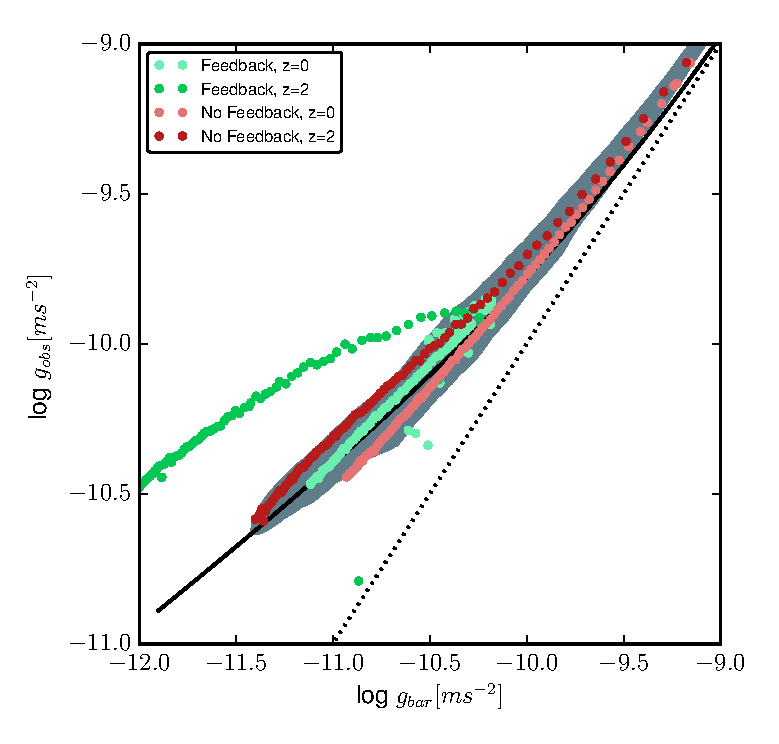
\includegraphics[width=0.6\textwidth]{figures4/FB_effects.eps}
    \caption[Feedback effects on acceleration relation]{The evolution seen in
    figure~\ref{redshift_evolution} is primarily driven by feedback.  This can
    be seen when looking at the same galaxy with and without feedback.  Without
    feedback, the baryon fraction within the disc increases slightly from $z=0$
    to $z=2$, but still roughly follows the SPARC relation.  At $z=2$, strong
    outflows in the galaxy expel most of the baryons from the disc, flattening
    the acceleration relation.  This effect is sensitive to the frequent
    merger-driven starbursts at high redshift, which can drive bursty outflows.}
    \label{FB_effects}
\end{figure}
If the SPARC acceleration law is in fact due to new physics, it would be
surprising if the law did not hold at all redshifts.  This would not be the case
if the relation was simply a consequence of galaxy evolution.  In
figure~\ref{redshift_evolution} we show that the acceleration relation in the MUGS2
sample actually shows significant redshift dependence, and only settles to
the equation~\ref{g_fit} relation near z=0.  For these data points, we scaled
the thickness of the annuli by the cosmic scale factor $a$, so that $\delta r =
300a\pc$.  We use this scaling to ensure we are sampling primarily from the
stellar disc, and not well beyond it.  Omitting this scaling has little effect
on these results, save for extending the points to very low values of $g_{bar}$
and removing points from the high $g_{bar}$ end.  This evolution is a
consequence of the huge impact that stellar feedback has on galaxies at
$z\sim2$.  \citet{Keller2015} showed that SNe drive hot outflows from high
redshift galaxies with mass loadings of $\dot M_{out}/\dot M_* \sim 10$.  This
leads to discs at high redshift with baryon fractions depleted relative to those at
low redshift.  This feedback effect is clear when a single galaxy, g1536, is
compared to the same galaxy simulated without SNe feedback.  As
figure~\ref{FB_effects} shows, the redshift trend is nearly nonexistent without SNe
feedback.  Even at $z=2$, the galaxy without feedback falls within the scatter
of the SPARC acceleration law, and within the scatter of the $z=0$ MUGS2
relation.  This tells us that we need not invoke feedback processes to explain
the SPARC acceleration law.  Simple dissipational collapse of gas is sufficient
to produce a similar relation.  The evolution we see as a function of redshift
is therefore dominated primarily by the stronger effect of feedback at higher
redshift.

\section{Discussion \& Conclusion}
We have shown here that the SPARC acceleration law can be produced by conventional
galaxy formation in a $\Lambda CDM$ universe.  Neither the particular functional
form (equation~\ref{g_fit}) nor the small scatter about this relation requires
anything beyond the dissipational collapse of baryons in a DM halo.  The fit
observed at $z=0$ does not hold at all redshifts: vigorous feedback at high
redshift acts to scour protogalaxies of their baryons, reducing the baryon
fraction of the disc, flattening the $g_{obs}-g_{bar}$ relation.  Stellar
feedback is an essential process if we are to produce realistic galaxies.  In order for
a single SPARC law to hold at all redshifts, feedback efficiencies would have to
be so low as to produce galaxies with stellar masses and bulge fractions in
conflict with the observed stellar mass to halo mass relation, and the observed
kinematics of local galaxies. If one wished to use equation~\ref{g_fit} to fit
galaxies at all epochs, $g_\dagger$ would need to have a significant redshift
dependence.  If, on the other hand, high redshift observations of the
$g_{obs}-g_{bar}$ relation found no evolution in shape, or a steeper slope at
low $g_{bar}$, this would in fact constitute a serious disagreement with
$\Lambda CDM$, as it would be difficult to produce the observed low cosmic star
formation efficiency without strong outflows removing baryons from high redshift
discs.

As figure~\ref{FB_effects} shows, the SPARC relation is {\it not} a result of
stellar feedback.  While feedback does change the relationship at high redshift,
its general form is reproduced by simple gas collapse and radiative cooling.
This is one of the few apparent problems in $\Lambda CDM$ that {\it doesn't}
require feedback for its resolution!

\section*{Acknowledgements}
We thank Hugh Couchman and Laura Parker for valuable discussion and suggestions.
The simulations used here were performed on the clusters hosted on
\textsc{scinet}, part of ComputeCanada.  We greatly appreciate the contributions
of these computing allocations.  We also thank NSERC for funding supporting this
research.  

\bibliographystyle{mnras}
\bibliography{library}
